%%%%%%%%%%%%%%%%%%%%%%%%%%%%%%%%%%%%%%%%%
% GU|CS Seminar/Project Thesis - Report version
% LaTeX Template
% Version 6.9 (2023/05/30)
%
% This version is the report version to keep track during the seminar progress.
%
% Original author:
% Debasish Dutta
%
%%%%%%%%%%%%%%%%%%%%%%%%%%%%%%%%%%%%%%%%%

%----------------------------------------------------------------------------------------
%	PACKAGES AND DOCUMENT CONFIGURATIONS
%----------------------------------------------------------------------------------------

\documentclass[report]{dd_dissertation} % Report version of the dissertation;
%\documentclass[final]{dd_dissertation} % Final version for submission;

\usepackage{dd_dissertation_pck}

%----------------------------------------------------------------------------------------
%	TITLE PAGE
%----------------------------------------------------------------------------------------

\begin{document}
\pagestyle{plain} % No page numbers
% \frontmatter % Use roman page numbering style (i, ii, iii, iv...) for the preamble pages

\puttitle{
	title=\LaTeX\ Seminar Report Title, % Title of the thesis
	degree=COMPUTER SCIENCE, % Degree Name
	name=Author Name, % Author name
	authordesignation=PS-XxX-xXx-XXXX, % Author designation
	supervisor=S.~Upervisor, % Supervisor name
	supervisordesignation=Supervisor Designation, % Supervisor designation  name
	submissionmonth={May 2023},  % Submission date "Month, year"
	submissiondate={20 May 2023}  % Submission date "Month, year"
}


%----------------------------------------------------------------------------------------
%	PREAMBLE PAGES (comment out unnecessary pages)
%----------------------------------------------------------------------------------------

\startpreamble

% \pagestyle{fancy} % Changes the headers
% \renewcommand{\chaptermark}[1]{ \markboth{#1}{}} % Getting the chapter name right
% \renewcommand{\sectionmark}[1]{\markright{\thesection\; #1}} % Getting the section name right
% \fancyhf{}% Clears header and footer
% \fancyhead[RO,LE]{\thepage} % page number on the outside of headers

% \begin{doublespacing}
% \unnumberedchapter{Certificate} 
\cleardoublepage
\thispagestyle{empty}

\begin{center}
 \textbf{\large DEPARTMENT OF COMPUTER SCIENCE}

  \vspace{0.2cm}
 \textbf{\LARGE GAUHATI UNIVERSITY}\\
 {\large GUWAHATI - 781014}\\
 {\large ASSAM}

 \vspace{1cm}

 \includegraphics[width=0.15\textwidth]{logo}

 \vspace{2cm}

 \textbf{\large CERTIFICATE}

 \vspace{2cm}

\end{center}

This is to certify that the seminar report entitled \textbf{\thesistitle} submitted by \textbf{\name}, for partial fulfilment for the requirement of award of the degree of Master of Science in \textbf{\degree}, Gauhati University is a work carried out by him under my supervision and guidance.

To the best of my knowledge, the work has not been submitted to any other institute for the award of any other degree or diploma.

 \vspace{3cm}

\begin{tabular}{p{8cm} c}
Date:	 \submissiondate &	\\
Place: Gauhati University	&\supervisor \\
	&	Supervisor\\
	&	\supervisordesignation\\
	&	Department of Computer Science\\
\end{tabular}


% \unnumberedchapter{Certificate} 
\cleardoublepage
\thispagestyle{empty}

\begin{center}
 \textbf{\large DEPARTMENT OF COMPUTER SCIENCE}

  \vspace{0.2cm}
 \textbf{\LARGE GAUHATI UNIVERSITY}\\
 {\large GUWAHATI - 781014}\\
 {\large ASSAM}

 \vspace{1cm}

 \includegraphics[width=0.15\textwidth]{logo}

 \vspace{2cm}

 \textbf{\large CERTIFICATE}

 \vspace{2cm}

\end{center}

This is to certify that the project report entitled \textbf{\thesistitle} submitted by \textbf{\name}, for partial fulfilment for the requirement of award of the degree of Master of Science in \textbf{\degree}, Gauhati University is a work carried out by him under my supervision and guidance.

To the best of my knowledge, the work has not been submitted to any other institute for the award of any other degree or diploma.

 \vspace{3cm}

\begin{tabular}{p{8cm} c}
Date:	 \submissiondate & \supervisor \\
Place: Gauhati University	& Supervisor \\
	&	Department of Computer Science \\
	% &	\supervisordesignation\\
	&	\\
\end{tabular}


% \unnumberedchapter{Certificate} 
\cleardoublepage
\thispagestyle{empty}

\begin{center}
 \textbf{\large DEPARTMENT OF COMPUTER SCIENCE}

  \vspace{0.2cm}
 \textbf{\LARGE GAUHATI UNIVERSITY}\\
 {\large GUWAHATI - 781014}\\
 {\large ASSAM}

 \vspace{1cm}

 \includegraphics[width=0.15\textwidth]{logo}

 \vspace{2cm}

 \textbf{\large CERTIFICATE}

 \vspace{2cm}

\end{center}

The project report entitled \textbf{\thesistitle} submitted by \textbf{\name}, for partial fulfilment for the requirement of award of the degree of Master of Science in \textbf{\degree}, Gauhati University has been examined.


 \vspace{5cm}

\begin{tabular}{p{8cm} c}
Date:	 \submissiondate & \supervisor \\
Place: Gauhati University	& Supervisor \\
	&	Department of Computer Science \\
	% &	\supervisordesignation\\
	&	\\
\end{tabular}


% \unnumberedchapter{Declaration}
\cleardoublepage
\thispagestyle{empty}

\vspace*{2cm}

\begin{center}


  \textbf{\large DECLARATION}

  \vspace{5cm}

\end{center}

I hereby declare that the seminar report entitled \textbf{\thesistitle}has been compiled by me and
submitted in partial fulfilment for the requirement of award of the degree of \textbf{Master of Science in Information Technology}, Gauhati University. I also declare that any or all contents incorporated in
the report has not been submitted in any form for the award of any other degree of any other institute or university.

 \vspace{5cm}

\begin{tabular}{p{8cm} p{15cm} l}
Date: \submissiondate & \\
Place: Gauhati University		&	\name \\
&	Roll No.: \authordesignation\\
	&	Programme: Computer Science\\
	&	Semester: Fourth Semester\\

\end{tabular}
% \unnumberedchapter{Declaration}
\cleardoublepage
\thispagestyle{empty}

\vspace*{2cm}

\begin{center}


  \textbf{\large ACKNOWLEDGEMENT}

  \vspace{5cm}

\end{center}

\noindent
I acknowledge and express my gratitude to my project guide, \textbf{Dr Irani Hazarika}, Assistant
Professor, Department of Computer Science, Gauhati University, for her unwavering support, encouragement
and valuable advice throughout this project. Her expertise and guidance helped shape the
direction of my work. \\
I also extend my sincere thanks to \textbf{Prof. Anjana Kakoti Mahanta}, Department
of Computer Science, Gauhati University, for her support in this project. Her insights and inputs
have been invaluable in enhancing the quality of my work. \\
I would like to express my gratitude to all the faculty members of the Computer Science Department, Gauhati University, for their support and
encouragement throughout this project. 

 \vspace{5cm}

\begin{tabular}{p{12cm} p{15cm} l}
  Date: \submissiondate  &	\name \\
  % Place: Gauhati University	 &	Roll No.: \authordesignation\\
	% &	Programme: Computer Science\\
	% &	Semester: Fourth Semester\\

\end{tabular}
% \end{doublespacing}
% \unnumberedchapter{Abstract} 
\chapter*{Abstract} 
\subsection*{\thesistitle}

The abstract must fit in one page.
% \unnumberedchapter{Abbreviations} 
\chapter*{Abbreviations} 

Contains all abbr. used in the dissertation.

Here is an example.

\begin{longtable}{rl}
PPT & positive partial transpose\\
SRPT & Schr\"odinger-Robertson partial transpose
\end{longtable}
% \unnumberedchapter{Glossary} 
\chapter*{Glossary} 


Here is an example:

% Break up this table into several ones if it takes up more than one page
\begin{center}
\begin{longtable}{r p{0.58 \textwidth}}
Dipole Blockade & Phenomenon in which the simultaneous excitation of two atoms is inhibited by their dipolar interaction. \\
Cavity Induced Transparency & Phenomenon in which a cavity containing two atoms excited with light at a frequency halfway between the atomic frequencies contains the number of photons an empty cavity would contain.  \\ 
\end{longtable}
\end{center}


%----------------------------------------------------------------------------------------
%	LIST OF CONTENTS/FIGURES/TABLES
%----------------------------------------------------------------------------------------

% \unnumberedchapter{Contents}
% \tableofcontents % Write out the Table of Contents
% \unnumberedchapter{List of Figures}
% \listoffigures % Write out the List of Figures
% \unnumberedchapter{List of Tables}
% \listoftables % Write out the List of Tables
% \unnumberedchapter{List of Listings}
% \addcontentsline{toc}{section}{List of Listings}
% \lstlistoflistings
% \newpage
%----------------------------------------------------------------------------------------
%	THESIS MAIN TEXT - CHAPTERS
%----------------------------------------------------------------------------------------

% \addtocontents{toc}{\vspace{2em}} % Add a gap in the Contents, for aesthetics
% \mainmatter % Begin numeric (1,2,3...) page numbering
% \doublespacing % Double spacing

\begin{abstract}
	This seminar report serves as a guide to using LaTeX, a powerful typesetting system. It provides explanations and examples for various LaTeX components.
\end{abstract}
	

% \numberedchapter
\section{Introduction on how to use this template}
LaTeX is a typesetting system commonly used for producing high-quality documents, including research papers, reports, and presentations. It offers several advantages over traditional word processors. In this seminar, we'll explore some essential LaTeX components.

This is a practical guide into how to use this template, by explaining the role of the different folders and files.

If some practices seem like overkill for a 20 page proposal (splitting the content across different files), that is because it probably is, but we built it this way because this thesis template is structured identically. That means that you will be able to incorporate this document into your thesis seamlessly.

\section{Template Structure}


\subsection{Folder Setup}
The main folder contains three folders detailed here:
\begin{itemize}

    \item \textbf{Assets.} This folder should contain all the images that you will use in your thesis. It can contain subfolders, for example one for each chapter. To include an image from the main text, use something like \texttt{\textbackslash includegraphics\{subfolder/image.jpg\} } without worrying about the \texttt{Images} path.

    \item \textbf{MainText.} This folder contains a series of \LaTeX\ files that form the main text: introduction, chapters, conclusion, appendices and published articles. The introduction and conclusion as they are now are not numbered, which creates a few difficulties with the headers of the thesis. Those are solved by including the commands \texttt{\textbackslash unnumberedchapter\{\}} and \texttt{\textbackslash numberedchapter} before including the files in \texttt{xxx\_Thesis.tex}. If you want the introduction and conclusion to be numbered, re-write and treat them as regular chapters.
    
    \item \textbf{Preamble.} This folder contains a series of \LaTeX\ files with the pages that will appear before the main text. These files are mainly for the final dissertation. Do not modify them for unless neccessary. The files are:
    \begin{itemize}
    \item \texttt{abstract.tex} --- Abstract. Follow directions in the file.
    \item \texttt{certificate\_ext.tex} --- Acknowledgments. Follow directions in the file.
    \item \texttt{certificate\_hod.tex} --- Acknowledgments. Follow directions in the file.
    \item \texttt{certificate.tex} --- Acknowledgments. Follow directions in the file.
    \item \texttt{declaration.tex} --- Declaration of Original and Sole Authorship. Only modify the last item. This page needs to be signed once printed.
    \item \texttt{glossary.tex} --- Glossary (optional). If the list goes over one page, create another table.
    \item \texttt{apa.bst} --- Bibliography style file modified to suit this thesis. If you want to use another custom bibliography style, include the file in this folder.
    \item \texttt{Thesis\_bibliography.bib} --- BibTeX file containing your bibliography.
    \item \texttt{report\_bib.bib} --- BibTeX file containing your bibliography for reports.
    \end{itemize}
    
    \end{itemize}

\subsection{\texttt{Report.tex}}

    This is the main file, the only one that need to be compiled to build the document. Compile once with \LaTeX, once with BibTeX and finally twice with \LaTeX\ to get all the references right.
    
    Let's go through each section and comment them briefly. \cite{App88} The last section will emphasize the differences between the two files.\cite{C_grammar}
    

\subsection{Differences between a report version and final version}

    There are two main differences between \verb|\documentclass[report]{dd_dissertation}| and \verb|\documentclass[final]{dd_dissertation}|. 
    
    The difference is in the document style: page size, header and line spacing are different This might create small issues, such as page breaking with large tables, images or captions, when compiling the same content.
    

\section{Document Structure}
\subsection{Title, Author, and Date}
To set the title, author, and date, change the \texttt{title}, \texttt{author}, and \texttt{date} commands:
\begin{verbatim}
title=Seminar Report: A Guide to LaTeX,
name=Author Name,
authordesignation=PS-XxX-xXx-XXXX,
supervisor=Supervisor name, 
supervisordesignation=Supervisor Designation, 
submissionmonth={May 2023}  


\end{verbatim}
\section{Text Formatting}
\subsection{Sections and Subsections}
Divide your document into sections and subsections using the \texttt{section} and \texttt{subsection} commands:
\begin{verbatim}
\section{Introduction}
\subsection{Document Class}
\end{verbatim}
\subsection{Emphasis}
Use \texttt{emphasized text} for emphasizing text and \textbf{bold text} for making text bold.

\section{Lists, Figures, Tables and Codes}
\subsection{Lists}
\subsubsection{Unordered Lists}
Create bullet-point lists using the \texttt{itemize} environment:
\begin{itemize}
  \item Item 1
  \item Item 2
\end{itemize}

\subsubsection{Ordered Lists}
Create numbered lists using the \texttt{enumerate} environment:
\begin{enumerate}
  \item First item
  \item Second item
\end{enumerate}

\subsection{Figures}
Insert figures using the \texttt{figure} environment:
\begin{figure}[H]
  \centering
  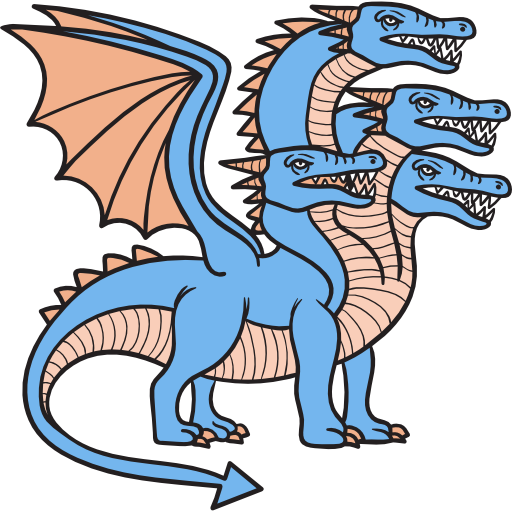
\includegraphics[width=0.25\textwidth]{chap3/dragon.png} 
  \caption{A sample figure.}
  \label{fig:sample}
\end{figure}

Refer to figure like this: Figure~\ref{fig:sample} or this (Fig.~\ref{fig:sample}). 


\subsection{Tables}
\begin{table}[H] 
    \center
    \caption{Short heading above the table.}
    \begin{tabular}{c|c}
    Parameter & Value \\ \hline \hline
    $\Delta$ & 0, 150 \\
    ${\alpha}$ & 85 \\
    ${\epsilon}$ & 6 \\
    ${\kappa}$ & 6.8 \\
    ${\gamma}$ & 0.2
    \end{tabular}
    \label{tab:values}
    \caption*{Full caption with all the details here.}
    \end{table}
    
    \begin{table}[H] \center
    \begin{tabular}{c|c}
    Parameter & Value \\ \hline \hline
    $\Delta$ & 0, 1500 \\
    ${\alpha}$ & 850 \\
    ${\epsilon}$ & 60 \\
    ${\kappa}$ & 68 \\
    ${\gamma}$ & 2
    \end{tabular}
    \caption{This is how tables are created}
    \end{table}
    
    
    Refer to tables this this: Table~\ref{tab:values}.

    \subsection{Codes}

    \begin{lstlisting}[caption={My Captions},captionpos=b]
        x := -2 + y
        
        \end{lstlisting}
       
    \begin{lstlisting}[language=C,caption={[short caption]caption text}, captionpos=b]
                     int main() {
                         //compound statement #1 
                         int a = 1;
                         {       
                             //compound statement #2
                             a = 2;
                                 if (a) {
                                     //compound statement #3
                                     a = 4;
                             }
                         }
                     }
            
            \end{lstlisting}
    
    \pagebreak
    For indented code insertation we can do it like this.
    \begin{verbatim}
        // Hello.java
        import javax.swing.JApplet;
        import java.awt.Graphics;
    
        public class Hello extends JApplet {
            public void paintComponent(Graphics g) {
                g.drawString("Hello, world!", 65, 95);
            }    
        }
    
        \end{verbatim}


\section{References}
Cite references using the \texttt{cite} command:
\begin{verbatim}
According to \cite{author2022}, LaTeX is powerful.
\end{verbatim}

\section{Conclusion}
This seminar report provides a brief introduction to LaTeX and some of its essential components. Experiment with LaTeX to create beautiful documents.

 % Import your chapters here
% \chapter{Introduction}\label{ch-1} 
% \chapter{How to use the template} \label{ch-2}

This is a practical guide into how to use this template, by explaining the role of the different folders and files.

If some practices seem like overkill for a 20 page proposal (splitting the content across different files), that is because it probably is, but we built it this way because this thesis template is structured identically. That means that you will be able to incorporate this document into your thesis seamlessly.

\section{Folders}

The main folder contains three folders detailed here:

\begin{itemize}

    \item \textbf{Assets.} This folder should contain all the images that you will use in your thesis. It can contain subfolders, for example one for each chapter. To include an image from the main text, use something like \texttt{\textbackslash includegraphics\{subfolder/image.jpg\} } without worrying about the \texttt{Images} path.

    \item \textbf{MainText.} This folder contains a series of \LaTeX\ files that form the main text: introduction, chapters, conclusion, appendices and published articles. The introduction and conclusion as they are now are not numbered, which creates a few difficulties with the headers of the thesis. Those are solved by including the commands \texttt{\textbackslash unnumberedchapter\{\}} and \texttt{\textbackslash numberedchapter} before including the files in \texttt{xxx\_Thesis.tex}. If you want the introduction and conclusion to be numbered, re-write and treat them as regular chapters.
    
    \item \textbf{Preamble.} This folder contains a series of \LaTeX\ files with the pages that will appear before the main text. Please write (or copy and paste) your own text in those files and delete the dummy text when appropriate. The files are:
    \begin{itemize}
    \item \texttt{abbreviations.tex} --- List of abbreviations. If the list goes over one page, create another table.
    \item \texttt{abstract.tex} --- Abstract. Follow directions in the file.
    \item \texttt{certificate.tex} --- Acknowledgments. Follow directions in the file.
    \item \texttt{declaration.tex} --- Declaration of Original and Sole Authorship. Only modify the last item. This page needs to be signed once printed.
    \item \texttt{glossary.tex} --- Glossary (optional). If the list goes over one page, create another table.
    \item \texttt{physics\_bibstyle.bst} --- Bibliography style file modified by Jeremie Gillet in 2011 to suit his thesis. Might be suitable for physics. If you want to use another custom bibliography style, include the file in this folder.
    \item \texttt{Thesis\_bibliography.bib} --- BibTeX file containing your bibliography.
    \item \texttt{report\_bib.bib} --- BibTeX file containing your bibliography for reports.
    \end{itemize}
    
    \end{itemize}

\section{\texttt{Dissertation.tex}}

This is the main files, the only one that need to be compiled to build the document. Compile once with \LaTeX, once with BibTeX and finally twice with \LaTeX\ to get all the references right.

Let's go through each section and comment them briefly. \cite{App88} The last section will emphasize the differences between the two files.\cite{C_grammar}

\subsection{PACKAGES AND OTHER DOCUMENT CONFIGURATIONS}

This section contains the minimum number of packages and definitions to compile the thesis. No line should be removed or modified.

\subsection{ADD YOUR CUSTOM VALUES, COMMANDS AND PACKAGES}

This section should not be modified directly. Instead, your packages and definitions should be included in  \texttt{Preamble/mydefinitions.tex}.

\subsection{TITLE PAGE}

Creates the title page.

\subsection{PREAMBLE PAGES}

Structures the style (header) for the preamble pages and builds them. Do not modify.

\subsection{LIST OF CONTENTS/FIGURES/TABLES}

Creates the list of contents. Do not modify.

\subsection{THESIS MAIN TEXT}

Structures the style for the main text chapters and builds them. 

\subsection{BIBLIOGRAPHY}

Builds the bibliography. The style of the bibliography can be defined in \texttt{Preamble/mydefinitions.tex}.

\subsection{APPENDICES}

Structures the style for the appendices and builds them. The appendices are numbered with letters but are structured like regular chapters.

\subsection{Differences between a report version and final version}

There are two main differences between \verb|\documentclass[report]{dd_dissertation}| and \verb|\documentclass[final]{dd_dissertation}|. 

The difference is in the document style: page size, header and line spacing are different This might create small issues, such as page breaking with large tables, images or captions, when compiling the same content.

 
% \chapter{Figures, tables and images} \label{chap-3}

\section{Figures}

\begin{figure}
\center
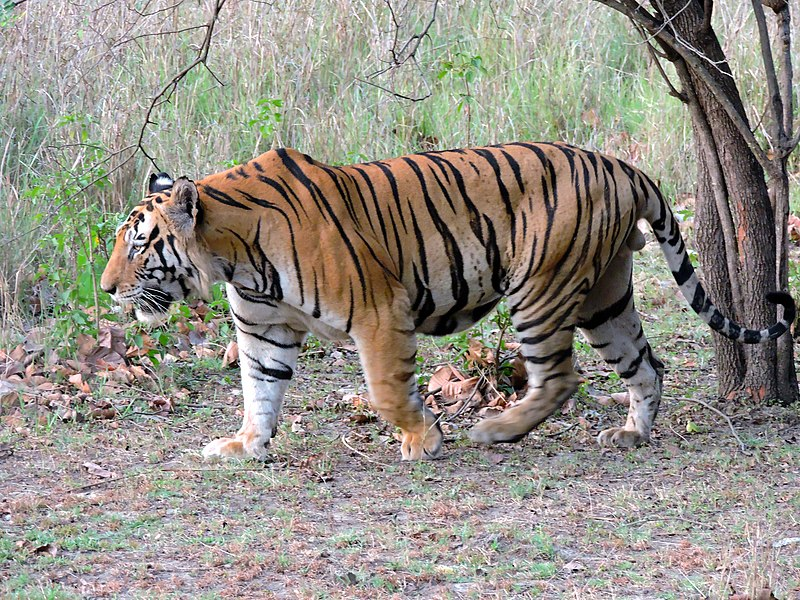
\includegraphics[width=0.3\textwidth]{chap3/tiger.jpg} 
\caption[Short caption for List of Figures]{{\bfseries Short caption (if wanted).} Full caption with all the details here.}
\label{fig-example}
\end{figure}

\begin{figure}
\center
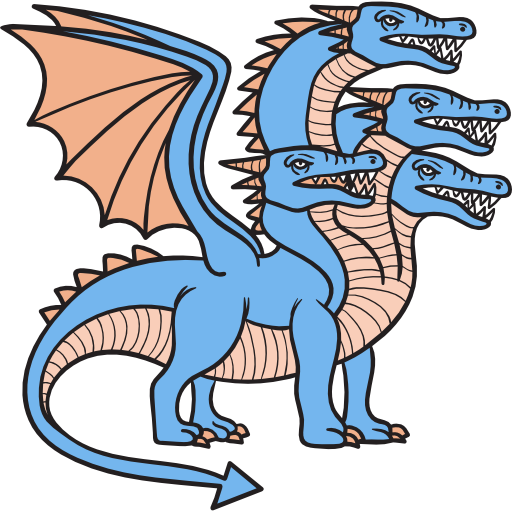
\includegraphics[width=0.3\textwidth]{chap3/dragon.png} 
\caption*{This secret image won't be numbered and won't appear in the List of Figures because of the *}
\end{figure}

Refer to figure like this: Figure~\ref{fig-example} or this (Fig.~\ref{fig-example}). If you want to include a list of figure, you can use a short version of the caption as shown in Figure~\ref{fig-example}.


\section{Tables}

\begin{table} 
\center
\caption{Short heading for the List of Tables.}
\begin{tabular}{c|c}
Parameter & Value \\ \hline \hline
$\Delta$ & 0, 150 \\
${\alpha}$ & 85 \\
${\epsilon}$ & 6 \\
${\kappa}$ & 6.8 \\
${\gamma}$ & 0.2
\end{tabular}
\label{tab-values}
\caption*{Full caption with all the details here.}
\end{table}

\begin{table} \center
\begin{tabular}{c|c}
Parameter & Value \\ \hline \hline
$\Delta$ & 0, 1500 \\
${\alpha}$ & 850 \\
${\epsilon}$ & 60 \\
${\kappa}$ & 68 \\
${\gamma}$ & 2
\end{tabular}
\caption*{This secret table won't be numbered and won't appear in the List of Figures because of the * }
\end{table}


Refer to tables this this: Table~\ref{tab-values}. 
% \chapter{Codes, timeline} \label{chap-4}

\section{Codes}

\begin{lstlisting}[caption={My Captions},captionpos=b]
    x := -2 + y
    
    \end{lstlisting}
   
\begin{lstlisting}[language=C,caption={[short caption]caption text}, captionpos=b]
                 int main() {
                     //compound statement #1 
                     int a = 1;
                     {       
                         //compound statement #2
                         a = 2;
                             if (a) {
                                 //compound statement #3
                                 a = 4;
                         }
                     }
                 }
        
        \end{lstlisting}

\pagebreak
For intext code insertation we can do it like this.
\begin{verbatim}
    // Hello.java
    import javax.swing.JApplet;
    import java.awt.Graphics;

    public class Hello extends JApplet {
        public void paintComponent(Graphics g) {
            g.drawString("Hello, world!", 65, 95);
        }    
    }

    \end{verbatim}

\pagebreak
\section{Timeline}

\begin{table}[h]
    \small{
    % \renewcommand\arrystretch{1.4}\arrayrulecolor{LightSteelBlue3}
    \captionsetup{singlelinecheck=false, font=blue, labelfont=sc, labelsep=quad}
    \caption{Timeline}\vskip -1.5ex
    \begin{minipage}[t]{.7\linewidth}
    \color{gray}
    \rule{\linewidth}{1pt}
    \ytl{10 Sept 2022} {Start\\}
    \ytl{16 Sept 2022} {Finish Primary Research\\}
    \ytl{19 Sept 2022} {Explore Problem Statement\\}
    \ytl{20 Sept 2022} {Criteria Selection\\}
    \ytl{23 Sept 2022} {Proposed Methodology\\}
    \ytl{30 Sept 2022} {Started Working Theoritical solution\\}
    \ytl{30 Oct 2022} {Started Working Practical solution\\}
    \ytl{05 Nov 2022}  {Submited progress report\\}
    \ytl{07 Nov 2022}  {Second Seminar\\}
    \ytl{25 Nov 2022}  {Finalize Literature review, Methodology and the Language Designing\\}
    \ytl{20 Dec 2022}  {Submit Progress Report to Guide\\}
    \bigskip
    \rule{\linewidth}{1pt}%
    \end{minipage}
    }%
\end{table} 
% \input{MainText/chapter5} 
% \input{MainText/chapter6} 
% \input{MainText/chapter7} 
% \input{MainText/chapter8} 
% \input{MainText/chapter9} 

\pagebreak
%----------------------------------------------------------------------------------------
%	BIBLIOGRAPHY
%----------------------------------------------------------------------------------------

% \addtocontents{toc}{\vspace{2em}} % Add a gap in the Contents, for aesthetics
% \unnumberedchapter{Bibliography} % Title of the unnumbered chapter
% \bibliography{./Preamble/Thesis_bibliography} % The references information are stored in the file named "Thesis_bibliography.bib"
\bibliography{Preamble/report_bib} % The references information are stored in the file named "report_bib.bib"

%----------------------------------------------------------------------------------------
%	APPENDICES
%----------------------------------------------------------------------------------------

% \addtocontents{toc}{\vspace{2em}} % Add a gap in the Contents, for aesthetics
% \appendix % Starts of appendices

% \numberedchapter
% \chapter{About Appendices}\label{appA}


Appendices are optional and should only be used if necessary.
% \chapter{Script}\label{appB}

The following file is used, hence can be imported directly from the file.
\lstinputlisting[nolol=true, language=Python]{Assets/script.py}



% \input{MainText/appendixC}

\end{document}  